\documentclass[11pt]{article}
\usepackage[T1]{fontenc}
\usepackage{lmodern}
\usepackage[margin=1in]{geometry}
\usepackage{amsmath,amssymb,amsthm,mathtools}
\usepackage{booktabs,array}
\usepackage{graphicx}
\usepackage{microtype}
\usepackage{xurl}
\usepackage[hidelinks]{hyperref}
\usepackage{enumitem}
\usepackage[font=small,labelfont=bf]{caption}
\hypersetup{pdftitle={Twelve Clebsch graphs and a new upper bound for the Ramsey multiplicity of K4},
  pdfauthor={Luke Van Seters and Madhan Jothimani}}
\newtheorem{theorem}{Theorem}[section]
\newtheorem{proposition}[theorem]{Proposition}
\newtheorem{lemma}[theorem]{Lemma}
\theoremstyle{definition}
\newtheorem{definition}[theorem]{Definition}
\theoremstyle{remark}
\newtheorem{remark}[theorem]{Remark}
\newcommand{\F}{\mathcal F}
\newcommand{\Z}{\mathbb Z}
\newcommand{\R}{\mathbb R}
\newcommand{\Q}{\mathbb Q}
\newcommand{\FF}{\mathbb F}
\newcommand{\code}[1]{\texttt{\detokenize{#1}}}
\setlength{\emergencystretch}{2em}
\setlist{itemsep=2pt,topsep=4pt}
\title{Twelve Clebsch graphs and a new upper bound\\ for the Ramsey multiplicity of $K_4$}
\author{Luke Van Seters \and Madhan Jothimani}
\date{October 3, 2026}

\begin{document}
\maketitle
\begin{abstract}
The Ramsey multiplicity constant $c_4$ is the smallest possible limiting density of monochromatic copies of $K_4$ in a red/blue coloring of $K_n$.
The best construction with public data, due to Parczyk, Pokutta, Spiegel, and Szab\'o (2022), is a Cayley graph on $768$ vertices with density $0.0301449$.
Their paper also reports an improvement by McKay to $0.0301423$ whose graph has not been released, and a 2026 seminar by Feinstein announced a construction below $0.030139$ without giving its value.
We show that the 768-vertex graph has a simple hidden structure: its vertices split into twelve families, each a fourfold blow-up of the Clebsch graph, and the colors between families follow one of four patterns according to a rule on $\Z_3\times\Z_2\times\Z_2$.
Making the fractional patterns adjustable gives a two-parameter step graphon on $192$ classes whose density is an explicit polynomial; its minimum, $0.03013898$, is already below McKay's value.
Refining this graphon with a pentagon pattern and two balanced sign splits gives a $3840$-class step graphon with exact density
\[
 U=\frac{8450462766487926638466333426306607129}{280384030360880691940646801777885184000}=0.0301388875665\ldots,
\]
so $c_4\le U$.
This is below Feinstein's announced threshold.
A rational point of the two-parameter family gives $c_4\le0.0301389941$ with a proof checked in Lean; the bound $U$ is established by an independent exact computation.
The constructions were found autonomously by OpenAI's GPT-6 Astra model running in the Codex harness, with one agent directing eight copies of itself as subagents.
\end{abstract}

\noindent\textbf{Keywords.} Ramsey multiplicity; Clebsch graph; step graphon; exact computation; formal verification; AI-assisted discovery.

\section{Introduction}
\label{sec:intro}

Color each edge of the complete graph $K_n$ red or blue.
How few monochromatic copies of $K_4$ can there be?
Let $m_4(n)$ be the minimum, over all colorings, of the proportion of four-vertex sets that span a monochromatic $K_4$, and let $c_4=\lim_{n\to\infty}m_4(n)$.
Coloring each edge by a fair coin gives $2\cdot2^{-6}=1/32$, so $c_4\le 1/32$.
For triangles, Goodman showed that the analogous random bound is sharp, $c_3=1/4$~\cite{goodman1959}, and Erd\H{o}s conjectured that random colorings are optimal for every clique~\cite{erdos1962}.
Thomason disproved this for $K_4$ and every larger clique~\cite{thomason1989}.
Determining $c_4$ remains open.

\paragraph{Upper bounds.}
Every explicit coloring, or more generally every step graphon (Section~\ref{sec:prelim}), gives an upper bound on $c_4$.
Figure~\ref{fig:bounds}(a) shows the history.
Thomason's 1989 construction gives $c_4<0.030304$~\cite{thomason1989}.
Franek and R\"odl found Cayley-graph constructions by computer with $c_4\le0.976501/32\approx0.030516$~\cite{franekrodl1993}.
Thomason improved his bound with graph products~\cite{thomason1997}, to $c_4<0.030291$ as reported in~\cite{ppss2025}, and Even-Zohar and Linial gave a composition construction with $c_4\le1411/46592\approx0.0302842$~\cite{evenzoharlinial2015}.
Jagger, \v{S}\v{t}ov\'{i}\v{c}ek, and Thomason showed more generally that every graph containing $K_4$ is \emph{uncommon}: some coloring beats the random one~\cite{jagger1996}.

\paragraph{Lower bounds.}
Giraud proved $c_4>1/46$~\cite{giraud1979}.
Razborov's flag algebra method~\cite{razborov2007} led to $c_4>1/34.79$ by Sperfeld~\cite{sperfeld2011} and $c_4>0.0287$ by Nie\ss~\cite{niess2012}.
Grzesik, Lee, Lidick\'y, and Volec remark that a flag algebra computation on nine-vertex graphs gives $c_4\ge0.0296$~\cite{grzesik2022}, and Kiem, Pokutta, and Spiegel report floating-point output suggesting $c_4\ge0.02961$~\cite[Section~7]{kiem2026}.
This paper is about upper bounds only.

\paragraph{The current frontier.}
Three recent results frame this work (Figure~\ref{fig:bounds}(b)).
\begin{enumerate}[leftmargin=*]
\item Parczyk, Pokutta, Spiegel, and Szab\'o (PPSS) searched over Cayley graphs and found a graph on $768$ vertices with
\[
 c_4\le\frac{4551721}{150994944}=0.0301448570\ldots
\]
\cite[Theorem~1.1]{ppss2025}.
The paper first appeared in 2022, and its graphs are publicly available~\cite{ppssdata2022}.
\item A later version of the same paper reports that McKay, starting from the PPSS graph and applying local search, found a $768$-vertex graph with density $10486266368/768^4=0.0301422734\ldots$~\cite[end of Section~5]{ppss2025}.
That graph has a trivial automorphism group, and we are not aware of a public copy.
\item In January 2026, Feinstein announced randomized constructions showing $c_4<0.030139$ in a seminar talk~\cite{feinstein2026}.
Neither the exact value nor the construction has been made public, as far as we know.
\end{enumerate}

\begin{figure}[tbp]
\centering
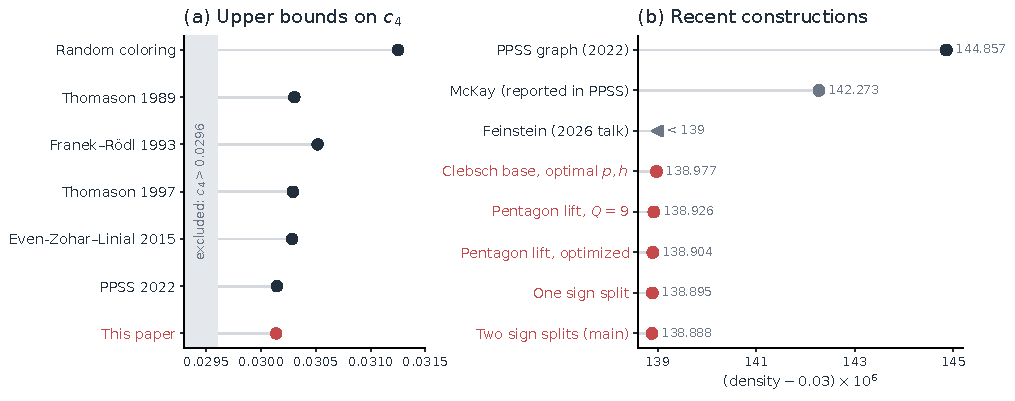
\includegraphics[width=\linewidth]{figures/bounds.pdf}
\caption{Upper bounds on $c_4$.
(a) Constructions since Thomason's disproof of the Erd\H{o}s conjecture; the shaded region is excluded by the flag algebra lower bound.
(b) A zoom on the recent constructions.
McKay's value is reported in~\cite{ppss2025} without public data, and Feinstein's announcement gives only the threshold $0.030139$.
Red points are the constructions of this paper.}
\label{fig:bounds}
\end{figure}

\paragraph{Our results.}
We start from the PPSS graph and make three contributions.

\emph{Structure.}
In its published form the PPSS graph is a $768\times768$ table of colors with little apparent pattern.
We show that it is built from the Clebsch graph, the strongly regular graph on $\FF_2^4$ with parameters $(16,5,0,2)$.
Its vertices split into $12$ families of $64$, each family into $16$ fibers of four vertices, and inside every family the blue edges form the Clebsch graph with each vertex replaced by four.
Between two families, the proportion of red edges between fibers follows one of four patterns, and which pattern applies is decided by a rule on the group $\Z_3\times\Z_2\times\Z_2$ (Section~\ref{sec:structure}, Figures~\ref{fig:clebsch}--\ref{fig:rule}).

\emph{A two-parameter family.}
Replacing the two fractional patterns by free probabilities $p$ and $h$ gives a step graphon $B_{p,h}$ with $192$ classes.
Its density is an explicit degree-six polynomial with a unique minimum $0.0301389773$ on $[0,1]^2$, already below McKay's value.
A nearby rational point gives Theorem~\ref{thm:compact}, which is proved in Lean.

\emph{Refinement.}
Splitting each class into five with a pentagon pattern, and then twice into two with balanced signs, lowers the density further (Section~\ref{sec:refinement}).
The result is our main theorem.

\begin{theorem}[Main bound]
\label{thm:main}
There is a symmetric $3840\times3840$ table $W_*$ of probabilities with denominator $65536$ such that
\begin{equation}
\label{eq:mainvalue}
 \F(W_*)=U=\frac{8450462766487926638466333426306607129}{280384030360880691940646801777885184000}=0.030138887566497220\ldots.
\end{equation}
Consequently, for every $n\ge4$ some red/blue coloring of $K_n$ has monochromatic $K_4$ proportion at most $U$, and $c_4\le U<0.030139$.
\end{theorem}

\begin{theorem}[Compact bound]
\label{thm:compact}
For $p=32/41$ and $h=22/41$,
\begin{equation}
\label{eq:compact}
 \F(B_{p,h})=U_{192}=\frac{1013294255057839}{33620705806123008}=0.030138994133588287\ldots,
\end{equation}
and therefore $c_4\le U_{192}$.
This statement, including the numerical evaluation, is proved in Lean.
\end{theorem}

Theorem~\ref{thm:main} improves the PPSS bound by $5.97\cdot10^{-6}$ and McKay's reported bound by $3.39\cdot10^{-6}$.
It is also below Feinstein's announced threshold.
Without an exact value for that construction we cannot say which is smaller, and we make no claim either way.

\paragraph{How the result was found.}
The decomposition, the two-parameter family, and both refinements were found by an autonomous research system: a parent GPT-6 Astra agent in OpenAI's Codex harness that directed eight GPT-6 Astra subagents, each pursuing a separate line of attack, under a research skill derived from published prompts for autonomous mathematics (Section~\ref{sec:methods}).
Every candidate the agents proposed was an explicit rational matrix, and none was accepted until a separate program had recounted it exactly.

\paragraph{Verification.}
Theorem~\ref{thm:compact} has an end-to-end formal proof in Lean.
For Theorem~\ref{thm:main}, Lean proves that the witness has the stated structure and that an optimized counting formula equals its density, but the final numerical evaluation is not yet formalized; the value in~\eqref{eq:mainvalue} comes from an independent exact computation based on a character identity (Section~\ref{sec:count}).
Section~\ref{sec:formal} states precisely what is proved and what is computed.

\section{Step graphons and finite colorings}
\label{sec:prelim}

An \emph{equal-class step graphon} on a finite index set $I$ with $|I|=N$ is a symmetric matrix $W=(w_{ij})_{i,j\in I}$ with entries in $[0,1]$~\cite{lovaszszegedy2006}.
We read $w_{ij}$ as the probability that an edge between a vertex of class $i$ and a vertex of class $j$ is red; the diagonal entry $w_{ii}$ describes edges between two distinct vertices of the same class.
The \emph{monochromatic $K_4$ density} of $W$ is
\begin{equation}
\label{eq:density}
 \F(W)=\frac1{N^4}\sum_{i_1,i_2,i_3,i_4\in I}
 \Bigl(\prod_{1\le s<t\le4}w_{i_si_t}+\prod_{1\le s<t\le4}(1-w_{i_si_t})\Bigr),
\end{equation}
which is $t(K_4,W)+t(K_4,1-W)$ in graphon notation.
The sum runs over all ordered quadruples, including those with repeated classes.

\begin{lemma}[Finite realization]
\label{lem:realization}
For every step graphon $W$ and every $n\ge4$, $m_4(n)\le\F(W)$.
Hence $c_4\le\F(W)$.
\end{lemma}
\begin{proof}
Give each vertex of $K_n$ an independent uniform class in $I$, then color each edge red independently with probability $w_{ij}$, where $i$ and $j$ are the classes of its ends.
For four distinct vertices, the four classes are independent and uniform (repetitions allowed) and the six edges are conditionally independent, so the probability that they span a monochromatic $K_4$ is exactly~\eqref{eq:density}.
The expected proportion of monochromatic four-sets is therefore $\F(W)$, and some coloring does at least as well.
Finally, $m_4(n)$ is nondecreasing, because averaging over the $n$-vertex subsets of an optimal coloring of $K_{n+1}$ shows $m_4(n)\le m_4(n+1)$; so $c_4$ exists and is at most $\F(W)$.
\end{proof}

When $w_{ij}=r_{ij}/Q$ with integers $r_{ij}$, put
\begin{equation}
\label{eq:integer}
 D(r)=\sum_{i_1,i_2,i_3,i_4\in I}\prod_{s<t}r_{i_si_t},
 \qquad\text{so that}\qquad
 \F(W)=\frac{D(r)+D(Q-r)}{N^4Q^6}.
\end{equation}
All exact values in this paper are computed this way, in integer arithmetic.
A finite graph is the special case of a $0/1$ table with zero diagonal, so the PPSS value is $\F$ of its adjacency matrix.

\section{The Clebsch structure of the PPSS graph}
\label{sec:structure}

\subsection{The Clebsch graph}

Let $V=\FF_2^4$ with standard basis $e_1,\dots,e_4$, and put
\[
 S=\{e_1,e_2,e_3,e_4,\;e_1+e_2+e_3+e_4\},\qquad C=\{0\}\cup S.
\]
The Clebsch graph is the Cayley graph on $V$ with connection set $S$: two binary strings are adjacent when they differ in exactly one coordinate or in all four (Figure~\ref{fig:clebsch}).
It is $5$-regular, adjacent vertices have no common neighbor, and nonadjacent vertices have exactly two.
In particular it is triangle-free.
The five neighbors of any vertex form an independent set, and the ten non-neighbors induce the Petersen graph.

If the Clebsch edges are colored blue and all other pairs red, blue has no triangle and so no $K_4$.
Red, however, contains many copies of $K_4$, so a single Clebsch coloring is far from optimal.
The point of the PPSS graph, as we now explain, is how twelve such colorings are coupled.

\begin{figure}[tbp]
\centering
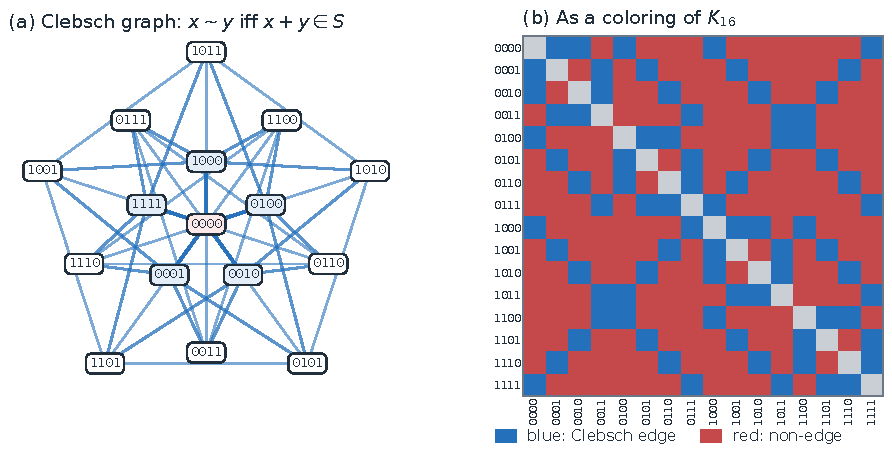
\includegraphics[width=0.92\linewidth]{figures/clebsch-graph.pdf}
\caption{The Clebsch graph on $\FF_2^4$.
(a) The vertex $0000$ is in the center, its five neighbors $S$ around it, and its ten non-neighbors outside.
(b) The same graph as a coloring of $K_{16}$, with Clebsch edges blue.
This $16\times16$ pattern reappears throughout Figures~\ref{fig:ppss} and~\ref{fig:rule}.}
\label{fig:clebsch}
\end{figure}

\subsection{Reading the PPSS graph}

Let $H=\Z_3\times\Z_2\times\Z_2$, whose elements $u=(a,e,s)$ will index twelve \emph{families}.
For two families put $u-v=(d_a,d_e,d_s)$ and define the \emph{type}
\begin{equation}
\label{eq:types}
 T(u,v)=
 \begin{cases}
 Z, & d_s=0,\ d_a=0,\ d_e=0 \quad(\text{the same family}),\\
 H, & d_s=0,\ d_a=0,\ d_e=1,\\
 X, & d_s=0,\ d_a\ne0,\ d_e=0,\\
 P, & d_s=1,\ d_a=0,\\
 Z, & \text{otherwise}.
 \end{cases}
\end{equation}
The type depends only on $u-v$, and $T(u,v)=T(v,u)$.
Each family is of type $H$ with one other family, of type $X$ with two, of type $P$ with two, and of type $Z$ with the remaining six.
Figure~\ref{fig:rule}(b) draws this as a graph on the twelve families: for each $a\in\Z_3$ the four families $(a,e,s)$ form a $K_4$ whose perfect matching $\{d_e=1,d_s=0\}$ is of type $H$ and whose remaining four-cycle is of type $P$, and corresponding families in the three copies are joined by triangles of type $X$.

Each type comes with a pattern on $V$, recorded in Table~\ref{tab:types} and Figure~\ref{fig:rule}(c)--(f).
Pattern $Z$ is the Clebsch coloring itself: blue at the same position and at Clebsch neighbors, red elsewhere.
Pattern $X$ is its complement.
Patterns $P$ and $H$ are fractional versions of $X$.

\begin{table}[tbp]
\centering
\caption{Red probability between position $x$ of family $u$ and position $y$ of family $v$, as a function of $z=x+y$ and the type $T(u,v)$.
The PPSS column is the proportion of red edges between the corresponding fibers of the PPSS graph; the last column is the two-parameter table $B_{p,h}$.
In the PPSS graph the same-position $P$ entry is $1$ when $d_e=0$ and $3/4$ when $d_e=1$.}
\label{tab:types}
\begin{tabular}{@{}l ccc c ccc@{}}
\toprule
 & \multicolumn{3}{c}{PPSS fiber averages} && \multicolumn{3}{c}{$B_{p,h}$}\\
\cmidrule{2-4}\cmidrule{6-8}
Type & $z=0$ & $z\in S$ & $z\notin C$ && $z=0$ & $z\in S$ & $z\notin C$\\
\midrule
$Z$ & $0$ & $0$ & $1$ && $0$ & $0$ & $1$\\
$X$ & $1$ & $1$ & $0$ && $1$ & $1$ & $0$\\
$P$ & $1$ or $3/4$ & $3/4$ & $0$ && $p$ & $p$ & $0$\\
$H$ & $1/2$ & $1$ & $0$ && $h$ & $1$ & $0$\\
\bottomrule
\end{tabular}
\end{table}

\begin{proposition}[Structure of the PPSS graph]
\label{prop:ppss}
The $768$ vertices of the PPSS graph~\cite{ppssdata2022} can be labeled bijectively by $H\times V\times\{1,2,3,4\}$ so that the following hold, where the fiber $(u,x)$ consists of the four vertices labeled $(u,x,\cdot)$.
\begin{enumerate}[label=(\roman*)]
\item Within a family $u$, an edge between vertices of fibers $(u,x)$ and $(u,y)$ is red if and only if $x+y\notin C$. In particular each fiber spans a blue $K_4$, and the blue graph inside a family is the Clebsch graph with each vertex replaced by a blue clique of size four.
\item For $u\ne v$, the proportion of red edges among the $16$ edges between fibers $(u,x)$ and $(v,y)$ is the PPSS entry of Table~\ref{tab:types} for type $T(u,v)$ and $z=x+y$.
\end{enumerate}
\end{proposition}

\begin{proof}
This is a finite check of all $768^2$ entries against an explicit labeling.
The labeling is stored with the repository, and the figure generator verifies (i) and (ii) every time it draws Figures~\ref{fig:ppss} and~\ref{fig:rule}.
\end{proof}

Figure~\ref{fig:ppss} shows the effect of the relabeling.
In the published vertex order the matrix shows little structure; in the new order it splits into a $12\times12$ grid of $64\times64$ blocks, the diagonal blocks are all the same blown-up Clebsch coloring, and every off-diagonal block is one of the four patterns.
The relabeling is only a permutation of the vertices, so the density is unchanged.

\begin{figure}[tbp]
\centering
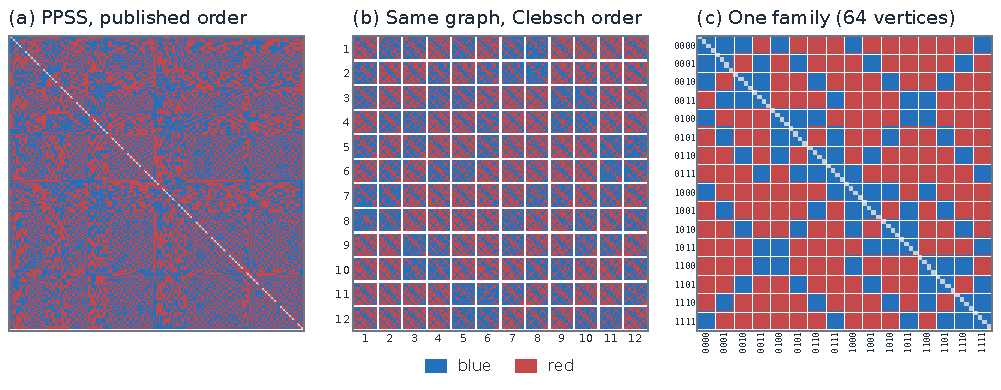
\includegraphics[width=\linewidth]{figures/ppss-reordered.pdf}
\caption{The PPSS graph~\cite{ppssdata2022} as a red/blue adjacency matrix.
(a) In the published vertex order.
(b) The same matrix with the vertices relabeled by Proposition~\ref{prop:ppss}: twelve families of $64$ vertices.
(c) One diagonal block: sixteen fibers of four vertices, colored by the Clebsch pattern of Figure~\ref{fig:clebsch}(b).
Gray marks the absent self-pairs.}
\label{fig:ppss}
\end{figure}

\begin{figure}[tbp]
\centering
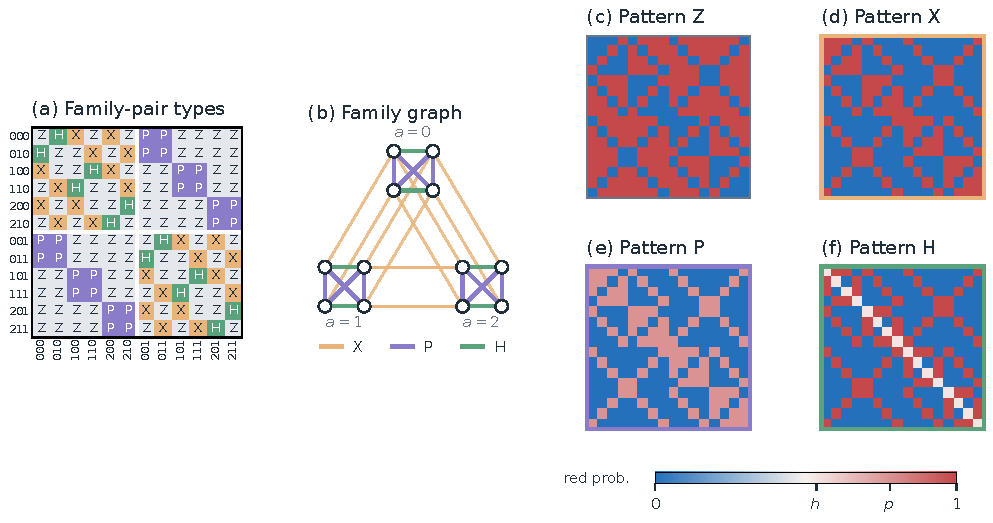
\includegraphics[width=\linewidth]{figures/family-rule.pdf}
\caption{The twelve-family rule.
(a) The type $T(u,v)$ for each pair of families, labeled $aes$ and ordered by $s$, then $a$, then $e$.
(b) The same rule as a graph on the families, omitting type $Z$.
(c)--(f) The four $16\times16$ position patterns, colored at the optimal parameters $p_*\approx0.779$ and $h_*\approx0.534$ of Proposition~\ref{prop:minimum}.
Pattern $Z$ is the Clebsch coloring and pattern $X$ its complement.}
\label{fig:rule}
\end{figure}

The two fractional patterns are where the PPSS graph uses finer structure than the Clebsch rule.
A $3/4$ block is the complement of a perfect matching between two fibers, and a $1/2$ block is a $2$-regular bipartite graph.
These $4\times4$ details matter: a direct count shows that the step graphon of fiber averages has density $9103117/301989888\approx0.0301438$, which is slightly smaller than the PPSS value but larger than McKay's.

Clebsch patterns are known to be extremal in neighboring problems.
Pikhurko and Vaughan show that blow-ups of the complement of the Clebsch graph minimize six- and seven-clique densities among graphs with independence number less than three~\cite{pikhurkovaughan2013}, and Kiem, Pokutta, and Spiegel determine the four-color triangle multiplicity through blow-ups of the two three-color Ramsey colorings of $K_{16}$, whose color classes are Clebsch graphs~\cite{kiem2026}.
We do not know of earlier work describing the PPSS graph in these terms.

\section{The two-parameter family}
\label{sec:base}

Proposition~\ref{prop:ppss} suggests replacing every fractional pattern by a free parameter.

\begin{definition}
For $p,h\in[0,1]$, let $B_{p,h}$ be the step graphon on the $192$ classes $I=H\times V$ given by
\begin{equation}
\label{eq:base}
 B_{p,h}((u,x),(v,y))=g_{T(u,v)}(x+y),
\end{equation}
where $g_Z,g_X,g_P,g_H\colon V\to[0,1]$ are the $B_{p,h}$ columns of Table~\ref{tab:types}.
\end{definition}

The table is symmetric, has zero diagonal, and is invariant under translation by the group $H\times V$ of order $192$.
Each row has $87$ entries equal to $1$, twelve equal to $p$, one equal to $h$, and $92$ equal to $0$.
Compared with the fiber averages of the PPSS graph, the $3/4$ and $1/2$ entries become $p$ and $h$, and the $96$ same-position $P$ pairs that were completely red also become $p$.

\begin{proposition}[Density polynomial]
\label{prop:poly}
$\F(B_{p,h})=P(p,h)/7077888$, where
\begin{equation}
\label{eq:poly}
\begin{aligned}
P(p,h)={}&251655-97344p+66888p^2-7008p^3+1224p^4\\
 &-6552h+9216ph-4176p^2h+2304p^3h-144p^4h\\
 &+990h^2-576ph^2+648p^2h^2-288p^3h^2+72p^4h^2\\
 &-16h^3+3h^4.
\end{aligned}
\end{equation}
\end{proposition}
\begin{proof}
Each summand of~\eqref{eq:density} is a polynomial in $p$ and $h$ of total degree at most six.
By translation invariance we may fix the first class to be the identity and divide by $192^3$.
Exact evaluation on the grid $\{0,1,\dots,6\}^2$ then determines the polynomial by interpolation; the supplement records the computation.
(Evaluations outside $[0,1]^2$ are used only as values of the polynomial.)
\end{proof}

Substituting $p=32/41$, $h=22/41$ gives~\eqref{eq:compact}, and Lemma~\ref{lem:realization} proves Theorem~\ref{thm:compact}.
The Lean proof evaluates the density directly and does not use the interpolation.
For comparison, $\F(B_{3/4,1/2})\approx0.0301467$ and $\F(B_{4/5,2/5})\approx0.0301418$; the second already improves on McKay's value.

\begin{proposition}[Minimum of the family]
\label{prop:minimum}
On $[0,1]^2$ the polynomial $P$ has a unique minimum, at
\[
 p_*=0.779180833031354\ldots,\qquad h_*=0.534265188030699\ldots,
\]
with value $\F(B_{p_*,h_*})=0.030138977289665338\ldots$.
The coordinates $p_*$ and $h_*$ are algebraic of degree seventeen.
\end{proposition}
\begin{proof}[Proof by exact computer algebra]
A lexicographic Gr\"obner basis of $(P_p,P_h)$ over $\Q$ has the form $\{h-r(p),g(p)\}$ with $g$ irreducible of degree seventeen (Appendix~\ref{app:minimum}).
A Sturm count shows that $g$ has exactly one real root, which lies in $(0,1)$, and root isolation puts the corresponding $h$ in $(0,1)$.
Interval evaluation gives $\F(B_{p_*,h_*})\in(0.03013897728966533,\,0.03013897728966535)$, and the Hessian there is positive definite (first diagonal entry above $0.01565$, determinant above $2.66\cdot10^{-6}$).
On the boundary, the edges $p=0$ and $p=1$ have no stationary points, the minima on $h=0$ and $h=1$ are approximately $0.0301635$ and $0.0301574$, and every corner value exceeds $0.03015$.
So the interior critical point is the unique global minimum.
\end{proof}

\section{Refinements}
\label{sec:refinement}

The minimum of Proposition~\ref{prop:minimum} is optimal only for $192$ classes.
Splitting each class into several equal subclasses, and letting the probabilities vary between subclasses while keeping their block averages, enlarges the family.
Because the density depends on products of six entries, a pattern with the same average can have a smaller density.
We use two such refinements (Figure~\ref{fig:refinement}).

\begin{figure}[tbp]
\centering
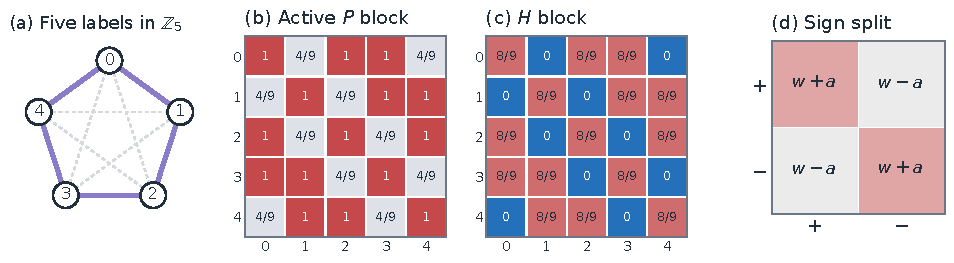
\includegraphics[width=\linewidth]{figures/refinements.pdf}
\caption{The two refinements.
(a) Each class is split into five subclasses indexed by $\Z_5$, and the pentagon $a-b=\pm1$ marks the \emph{on-pattern} pairs (here with phase $\gamma=0$).
(b) An active $P$ block of $C(9;7,4,8)$: $4/9$ on the pentagon and $1$ elsewhere, with every row and column averaging $7/9$.
(c) An $H$ block: $0$ on the pentagon and $8/9$ elsewhere, averaging $8/15$.
(d) A balanced sign split replaces an entry $w$ by a $2\times2$ block with the same average.}
\label{fig:refinement}
\end{figure}

\subsection{A pentagon refinement}

Replace each base class $i$ by five classes $(i,a)$, $a\in\Z_5$.
Blocks with value $0$ or $1$, including the diagonal blocks, stay constant.
Each of the $1248$ fractional pairs $i<j$ ($1152$ of type $P$ and $96$ of type $H$) receives a phase $\gamma_{ij}\in\Z_5$, or is marked inactive; we set $\gamma_{ji}=-\gamma_{ij}$.
A pair of subclasses $(i,a),(j,b)$ is on-pattern if $a-b-\gamma_{ij}\equiv\pm1\pmod5$.

For integers $Q,p_0,x,y$, the $960$-class table $C(Q;p_0,x,y)$ is:
\begin{itemize}
\item on an inactive $P$ pair, constant $p_0/Q$;
\item on an active $P$ pair, $x/Q$ on-pattern and $1$ otherwise;
\item on an $H$ pair, $0$ on-pattern and $y/Q$ otherwise.
\end{itemize}
In the phase table we use, $272$ of the $P$ pairs are inactive and the other $880$ are active.
The table is given as finite data in the supplement; we do not have a closed-form description of it.
Pentagon blow-ups also give the extremal colorings for three-color triangle multiplicity~\cite{cummings2013}, a different problem.

The simplest example uses only the probabilities $0,4/9,7/9,8/9,1$.
Two independent generic counters give
\begin{equation}
\label{eq:q9}
 \F(C(9;7,4,8))=\frac{4198776398959}{139314069504000}=0.030138925766\ldots,
\end{equation}
which is below the minimum of the two-parameter family.

For the optimized version, write the entries around their block means using the centered pentagon function
\[
 \kappa(d)=\begin{cases}3,&d\equiv\pm1,\\-2,&d\equiv0,\pm2,\end{cases}
 \qquad \sum_{d\in\Z_5}\kappa(d)=0.
\]
With $Q=65536$, an active $P$ pair has numerator $51064+q_{ij}\kappa(a-b-\gamma_{ij})$, an inactive one has $51064$, and an $H$ pair has $35139-11713\,\kappa(a-b-\gamma_{ij})$.
With $q_{ij}=-7236$ for every active pair this is $C(65536;51064,29356,58565)$.
The optimized table $W_0$ changes $q_{ij}$ on $234$ of the $880$ active pairs, to integers between $-7236$ and $-5685$, and has
\begin{equation}
\label{eq:parent}
 \F(W_0)=\frac{16900934504649027287619486865996291}{560768060721761383881293603555770368}=0.030138903565399090\ldots.
\end{equation}

\subsection{Balanced sign refinements}

Let $W$ be a step graphon on $I$ and $A$ a symmetric matrix with $|A_{ij}|\le\min(w_{ij},1-w_{ij})$.
The \emph{balanced sign refinement} of $W$ by $A$ is the step graphon on $I\times\{\pm1\}$ given by
\begin{equation}
\label{eq:sign}
 W'((i,s),(j,t))=w_{ij}+st\,A_{ij}.
\end{equation}
The bound on $A$ keeps every entry in $[0,1]$, and each $2\times2$ block has average $w_{ij}$.
Signed perturbations of this kind are standard in the study of graphon inequalities~\cite{lovasz2011,csoka2023}; here we apply one to a nonconstant table.

\begin{proposition}[Sign refinement identity]
\label{prop:sign}
With $q_{ij}=1-w_{ij}$, we have $\F(W')-\F(W)=T_3(A)+T_4(A)$, where
\begin{align}
\label{eq:t3}
 T_3(A)&=\frac4{N^4}\sum_{i,j,k,l}A_{ij}A_{jk}A_{ki}\,(w_{il}w_{jl}w_{kl}-q_{il}q_{jl}q_{kl}),\\
\label{eq:t4}
 T_4(A)&=\frac3{N^4}\sum_{i,j,k,l}A_{ij}A_{jk}A_{kl}A_{li}\,(w_{ik}w_{jl}+q_{ik}q_{jl}),
\end{align}
and both sums include repeated indices.
\end{proposition}
\begin{proof}
Fix classes $i,j,k,l$ and expand the product of the six red entries~\eqref{eq:sign}.
The four signs are independent and uniform, so the average of a monomial over the signs vanishes unless every vertex of $K_4$ has even degree in the corresponding edge set.
The nonempty even subgraphs of $K_4$ are its four triangles and its three four-cycles, which give~\eqref{eq:t3} and~\eqref{eq:t4} for red.
For blue every amplitude changes sign, which flips the triangle terms and leaves the cycle terms unchanged.
\end{proof}

In particular, scaling $A$ by $\epsilon$ gives $\F(W')=\F(W)+\epsilon^3T_3(A)+\epsilon^4T_4(A)$, with no linear or quadratic term.
So a direction that lowers the density after refinement can be invisible to any first- or second-order test in the unrefined class space.
This is why the refinements can go below the minimum of a family whose Hessian is positive definite.

Applying two successive sign refinements to $W_0$, with integer amplitudes over $65536$, gives tables with $1920$ and $3840$ classes.
Table~\ref{tab:values} lists all the constructions.

\begin{table}[tbp]
\centering
\caption{Constructions of this paper, all with exact densities.}
\label{tab:values}
\begin{tabular}{@{}lrl@{}}
\toprule
Construction & Classes & Density\\
\midrule
PPSS graph~\cite{ppss2025} & $768$ & $0.030144857035\ldots$\\
Fiber averages of the PPSS graph & $192$ & $0.030143780841\ldots$\\
$B_{32/41,22/41}$ (Theorem~\ref{thm:compact}) & $192$ & $0.030138994134\ldots$\\
$B_{p_*,h_*}$ (minimum, irrational) & $192$ & $0.030138977290\ldots$\\
$C(9;7,4,8)$ & $960$ & $0.030138925766\ldots$\\
Optimized pentagon refinement $W_0$ & $960$ & $0.030138903565\ldots$\\
First sign refinement & $1920$ & $0.030138895264\ldots$\\
Second sign refinement $W_*$ (Theorem~\ref{thm:main}) & $3840$ & $0.030138887566\ldots$\\
\bottomrule
\end{tabular}
\end{table}

\section{The 3840-class witness}
\label{sec:witness}

The witness $W_*$ is $192$ coarse classes, each split into $20$ subclasses (a pentagon label and two sign labels).
Order the coarse classes as $(a,e,s,x)\in\Z_3\times\Z_2\times\Z_2\times\FF_2^4$, encode $x$ as an integer in $\{0,\dots,15\}$, and put $i=64a+32e+16s+x$.
Let $Q=65536$ and $b_{ij}=Q\,B_{51064/Q,\,35139/Q}(i,j)$.
(Here $35139/Q$ is the mean of the refined $H$ blocks; it differs slightly from the best unrefined value $35015/Q$.)

For each of the $1248$ fractional pairs $i<j$, the supplement gives a $20\times20$ integer block $M_{ij}$; put $M_{ji}=M_{ij}^{\mathsf T}$, and let $M_{ij}$ be the constant block $b_{ij}$ when $b_{ij}\in\{0,Q\}$, including on the diagonal.
Then
\begin{equation}
\label{eq:witness}
 W_*((i,\alpha),(j,\beta))=\frac{M_{ij}(\alpha,\beta)}{Q},\qquad i,j\in\{0,\dots,191\},\ \alpha,\beta\in\{0,\dots,19\}.
\end{equation}
Every entry is an integer in $[0,Q]$, and every row and column of $M_{ij}$ sums to $20b_{ij}$, so $W_*$ refines $B_{51064/Q,35139/Q}$ with the same block averages.
The supplement checks these properties exactly.
The full matrix that was counted has SHA-256 identifier
\begin{center}
\small\code{05302cbc635e939cc41f4ba019cdcba80199b0b83563100bac0b1a0d9fff1a29};
\end{center}
the compact data use a permutation of the coarse classes, and the supplement checks every entry against that matrix.

\section{An exact count by characters}
\label{sec:count}

A direct evaluation of~\eqref{eq:density} for $N=3840$ has about $2\cdot10^{14}$ terms.
We use the sign symmetry of $W_*$ to reduce it.
Fourier methods already appear in the multiplicity analysis of Jagger, \v{S}\v{t}ov\'{i}\v{c}ek, and Thomason~\cite{jagger1996}; we give the specific identity we need.

\subsection{The character identity}

Changing either sign label of every class simultaneously leaves $W_*$ unchanged, so $G=\FF_2^2$ acts freely with $960$ orbits.
The checker verifies this on every entry before using it.
In general, let $G=\FF_2^k$ with $K=|G|$, and suppose the integer red table has the form
\[
 r((u,x),(v,y))=f_{uv}(x+y),\qquad u,v\in J,\ x,y\in G,
\]
with $|J|=n$, so $N=nK$.
For $c\in G$ let $\chi_c(x)=(-1)^{c\cdot x}$ and $\widehat f_c(u,v)=\sum_{z\in G}f_{uv}(z)\chi_c(z)$.
Fourier inversion gives
\begin{equation}
\label{eq:inversion}
 r((u,x),(v,y))=\frac1K\sum_{c\in G}\widehat f_c(u,v)\chi_c(x)\chi_c(y).
\end{equation}

\begin{proposition}[Character count]
\label{prop:character}
For $c=(c_{12},c_{13},c_{14},c_{23},c_{24},c_{34})\in G^6$ let
\[
 S(c)=\sum_{u_1,u_2,u_3,u_4\in J}\ \prod_{s<t}\widehat f_{c_{st}}(u_s,u_t),
\]
and let $\mathcal C\subseteq G^6$ be the set of labelings whose labels sum to zero at each vertex of $K_4$.
Then
\begin{equation}
\label{eq:character}
 D(r)=K^{-2}\sum_{c\in\mathcal C}S(c),
\end{equation}
and $\mathcal C=\{(a+b,\,a+d,\,b+d,\,a,\,b,\,d):a,b,d\in G\}$.
\end{proposition}
\begin{proof}
Substitute~\eqref{eq:inversion} into each of the six factors of $D(r)$, which contributes $K^{-6}$.
At vertex $s$ the product of the incident characters is $\chi$ of the sum of the incident labels, and summing over $x_s\in G$ gives $K$ if that sum is zero and $0$ otherwise.
The four vertex sums leave exactly the labelings in $\mathcal C$, with a factor $K^4$.
Solving the vertex conditions with $c_{23}=a$, $c_{24}=b$, $c_{34}=d$ gives the description of $\mathcal C$.
\end{proof}

The identity applies to red and blue separately.
For $k=2$ there are $64$ labelings in $\mathcal C$, which fall into eleven orbits under permutations of the four vertices.
Since every Fourier block is symmetric, $S$ is constant on orbits, so we compute one representative per orbit.
Repeated coarse labels are included in every sum.

\subsection{Arithmetic and validation}

Each $S(c)$ is computed modulo several primes $p<2^{21}$ and reconstructed by the Chinese remainder theorem.
The product of the primes exceeds twice the bound
\begin{equation}
\label{eq:crtbound}
 |S(c)|\le n^4\prod_{s<t}\max_{u,v}|\widehat f_{c_{st}}(u,v)|,
\end{equation}
so the residues determine $S(c)$ as a signed integer.
The modular contractions run in C++ with Apple Accelerate matrix multiplication on residues below $p$.
The code checks that $n(p-1)^2<2^{53}$, so every dot product is an integer represented exactly in double precision, and reduces modulo $p$ after each product.

Before the full count, the checker confirms the shape, symmetry, range, and equal class weights of the input, and the sign symmetry and Fourier reconstruction on all $14745600$ entries.
It agrees with literal arbitrary-precision counts on $27$ small cases, including tables with arbitrary diagonals and without sign structure, and on principal submatrices of orders $480$ and $960$.
On the $1920$-class table it agrees with a full generic count in multiword integer arithmetic.
For $W_*$ it gives
\begin{align}
\label{eq:rawcounts}
 D(r)&=259147196226119060009588075500947710392320,\notag\\
 D(Q-r)&=260049236146899152657783450211330231613440,\notag\\
 N^4Q^6&=17226794825372509712833339501233265704960000,
\end{align}
which by~\eqref{eq:integer} is the value $U$ in~\eqref{eq:mainvalue}.
Lemma~\ref{lem:realization} then gives Theorem~\ref{thm:main}.
The value predicted by the search code was compared with this count only after the count was complete.
A generic count of the full $3840$-class table, without the symmetry reduction, has not been run.

\section{Formal verification}
\label{sec:formal}

The Lean development defines the density~\eqref{eq:density} literally and proves Lemma~\ref{lem:realization} and the counting identity for Cayley tables.
For $B_{32/41,22/41}$ it evaluates the density exactly by native evaluation, which gives Theorem~\ref{thm:compact} together with the asymptotic statement $c_4\le U_{192}$.
There are no \code{sorry} placeholders and no assumed numerical certificates.

The witness $W_*$ is also embedded in Lean as its $1248$ fractional blocks together with the coarse group rule.
Native checks establish its dimensions, symmetry, range, and centered rows; general proofs establish the centered expansion, a sparse counting reduction, and the correctness of the stored contractions, giving an integer expression for $\F(W_*)$ with denominator $65536^6\cdot3840^4$.
What remains is a numerical certificate that this integer expression equals~\eqref{eq:mainvalue}.
Until then, Theorem~\ref{thm:main} rests on the exact computation of Section~\ref{sec:count}.

The general proofs use Lean's standard axioms and mathlib.
The native checks additionally trust the compiler and runtime.
The external count trusts Python integer arithmetic, the C++ program, and the stated exactness bounds for Accelerate.
Jeong, Park, Hyun, Oum, and Yang formalize flag algebras in Lean with a certificate-to-proof compiler~\cite{jeong2026}; that work concerns lower-bound certificates, whereas our proofs realize explicit tables.

\section{How the construction was found}
\label{sec:methods}

The results in this paper were found by an autonomous AI research system.
Every agent was OpenAI's GPT-6 Astra model~\cite{astra2026}, running in OpenAI's Codex agent harness~\cite{codex}.
A parent agent ran the campaign and directed eight subagents, created with Codex's native subagent mechanism.
Each subagent worked on its own line of attack, such as new constructions, algebraic descriptions, optimization, literature review, and verification.
The parent kept a registry of approaches, combined the evidence, reassigned subagents as lines succeeded or failed, and decided which candidates to promote.

All agents followed a hypothesis-driven research skill, a set of standing instructions loaded into the harness.
We derived the skill from two public prompts for autonomous mathematical research: OpenAI's prompt for the Cycle Double Cover conjecture~\cite{cdcprompt} and the Jacobian Conjecture prompt hosted by Aaron Lou~\cite{jacobianprompt}.
From them it keeps diverse approach families, independent early work, a registry of approaches, concrete outputs, and adversarial review.
It adds what a computational search needs: falsifiable predictions, small-instance oracles, persistent experiment records, and independent exact recounts.
It drops the prompts' fixed agent counts and run lengths, and it permits literature searches.
The supplement contains the skill and a note on how it adapts the two prompts.

The path to Theorem~\ref{thm:main} went through the steps of this paper in order.
The fiber partition of the PPSS graph and its quotient on $192$ classes were found first, and a separate line of work then identified the quotient as the Cayley rule~\eqref{eq:types}.
Optimization of $p$ and $h$, the pentagon refinement, and the sign refinements followed, each improving the previous best.
The campaign started on 27 September 2026 at Sundai Hack~142~\cite{sundai2026}, and $W_*$ was produced and independently recounted within its first day.

The system was designed so that no agent could certify its own result.
Every proposed improvement was an explicit rational matrix with a hash and a predicted value, and was accepted only after a separate program had recounted it; the final count of $W_*$ was done by a checker that did not read the search code.
Agreement between agents was never treated as evidence.
The human authors are responsible for the paper and its claims, which rest on the proofs, the explicit witnesses, and the exact computations described above.

\section{Discussion}
\label{sec:discussion}

Most of the improvement over PPSS comes from the twelve-family Clebsch structure itself: two parameters reach $0.0301389773$, and the refinements lower this by a further $9.0\cdot10^{-8}$, of which the two sign splits contribute $1.6\cdot10^{-8}$.
The sign identity explains why such gains are possible: they are of third order in the refinement amplitudes and invisible in the unrefined parameter space.
We do not know whether further refinements of the same base continue to help, or whether a different number of families or a different base graph does better; in limited experiments, removing families made the density worse and adding families did not help.

Feinstein describes his constructions as structured and symmetric~\cite{feinstein2026}.
It would be interesting to know whether they are related to the Clebsch structure described here.

The gap to the lower bound $0.0296$ remains about $5\cdot10^{-4}$, far larger than any of the improvements above.
Narrowing it will likely require progress on the lower-bound side.
In a different normalization, Davey, Hurley, de Joannis de Verclos, Kang, and Volec find an exact Clebsch extremal case for a pentagon-counting problem using local flag algebras~\cite{davey2026}.

\section*{Data and code availability}

Code and data are at \url{https://github.com/lukevs/k4-ramsey}.
The \code{paper/} directory contains this manuscript, the compact construction data, and the verification records; Appendix~\ref{app:reproduction} lists the files.
The repository also contains the search programs, the independent counters, the Lean development, and the research records.

\section*{Acknowledgments}

This work began at Sundai Hack~142, \emph{Recursive Self Improvement and Formal Verification in Mathematics}, held at Harvard on 27 September 2026~\cite{sundai2026}.
Our biggest thanks go to the Sundai Club organizers: without the event, this work would not exist.
We especially thank Alejandro Zarzuelo Urdiales, a guest at the event, who selected the open problems for the hack from his Ulam Open Problems Difficulty Atlas and presented them to the participants; this problem was one of them.

We also thank Parczyk, Pokutta, Spiegel, and Szab\'o for publishing their construction data, which was the starting point of this work, and the authors of the two research prompts~\cite{jacobianprompt,cdcprompt}.

\appendix
\section{Supplement and reproduction}
\label{app:reproduction}

Paths are relative to \code{paper/} unless they start with \code{../}.
\begin{description}[style=nextline,leftmargin=1em,labelwidth=0pt]
\item[\code{data/final3840.json.gz}]
The coarse rule, the fractional block index, and all $1248$ blocks of $W_*$. It contains no density value.
\item[\path{../src/k4_ramsey/paper/witness.py}]
Checks the compact data (block means, range, sign symmetry) and can write the full integer table for an independent count.
\item[\code{data/final3840-audit.json}]
The character-count record: red and blue totals, primes, orbit representatives, bounds, and validation results.
\item[\code{data/base-polynomial.json}, \code{data/base-minimum.json}]
Coefficients of $P$, the elimination polynomials, root intervals, and boundary computations.
\item[\code{data/pentagon-q9.json.gz}]
The table $C(9;7,4,8)$ of~\eqref{eq:q9}, with its phase table, class map, and two independent count records.
\item[\code{data/research-workflow.md}, \code{data/workflow-source-principles.md}]
The research skill followed by all agents, and how it adapts the two source prompts.
\item[\code{data/manifest.json}]
Hashes of all supplement files.
\end{description}
From the repository root, \code{just paper-check} validates the supplement and \code{just paper-figures} regenerates the figures from the published data, rechecking Proposition~\ref{prop:ppss}.
The independent counter is \path{../research/experiments/round5_F5/zk_checker.py} with contraction engine \path{../research/experiments/round5_F5/k4mix.cpp}.
The Lean proof of Theorem~\ref{thm:compact} is in \path{../lean/K4Ramsey/Constructions/Clebsch192/Bound.lean}; the embedded witness is in \path{../lean/K4Ramsey/Constructions/Final3840/}.

The original full matrix orders fine labels as $20i+4a+2b+c$ with $a\in\{0,\dots,4\}$ and $b,c\in\{0,1\}$; the two sign changes act by the XOR masks $1$ and $2$ on the fine index.

\section{Elimination polynomial for the base minimum}
\label{app:minimum}

The primitive elimination polynomial for $p_*$ is
\begin{align*}
g(p)={}&288p^{17}-4968p^{16}+48528p^{15}-326808p^{14}+1640880p^{13}-6374994p^{12}\\
 &+19669380p^{11}-49113990p^{10}+100709306p^9-170524126p^8\\
 &+238109998p^7-272230472p^6+252306699p^5-183872508p^4\\
 &+106134988p^3-50525006p^2+20013641p-4856020.
\end{align*}
The supplement gives $h_*=r(p_*)$ with $r\in\Q[p]$ of degree sixteen, the elimination polynomial for $h_*$, and exact root intervals.

\bibliographystyle{plain}
\bibliography{references}
\end{document}
